% SC4040 --- Chapter 3: Online Algorithms (0->100 ground-up)
\chapter{Online Algorithms}
\label{ch:online}

\begin{quote}
\emph{``The future is uncertain --- decide now anyway, and bound your regret.''}
Online algorithms must commit without seeing what's next. Competitive analysis measures how much worse we do than an offline optimum that saw the whole sequence in advance.
\end{quote}

\noindent\fbox{\parbox{\dimexpr\linewidth-2\fboxsep-2\fboxrule}{%
\textbf{From zero: online vs.\ offline from daily life.} We motivate paging, renting, and hiring from everyday decisions before any definition. No prior online-algorithms background assumed.}}
\vspace{0.4em}

\section*{Learning Outcomes}
After this chapter you will be able to:
\begin{enumerate}[label=(L\arabic*)]
    \item define competitive ratio and $k$-competitiveness for online problems;
    \item prove LRU and FIFO are $k$-competitive for paging and no deterministic algorithm beats $k$;
    \item analyse the ski-rental problem and its $2$-competitive deterministic and $e/(e-1)$ randomised optima;
    \item solve the secretary problem and prove the $1/e$ success probability;
    \item apply potential-function and phase-partitioning techniques.
\end{enumerate}

% ============================================================
\section{Competitive Analysis: Grading Without Seeing the Exam}
\label{sec:competitive}

Offline optimum $\textsc{Opt}(\sigma)$ sees the whole request sequence $\sigma$. Online algorithm $\textsc{Alg}(\sigma)$ sees requests one-by-one and must decide irrevocably. For minimisation:
\[
\textsc{Alg}(\sigma)\le c\cdot\textsc{Opt}(\sigma)+\alpha\quad\forall\sigma,
\]
then $\textsc{Alg}$ is $c$-\emph{competitive} ($\alpha$ constant, often $0$). Smaller $c$ is better; $c=1$ means optimal.

\begin{figure}[h]\centering
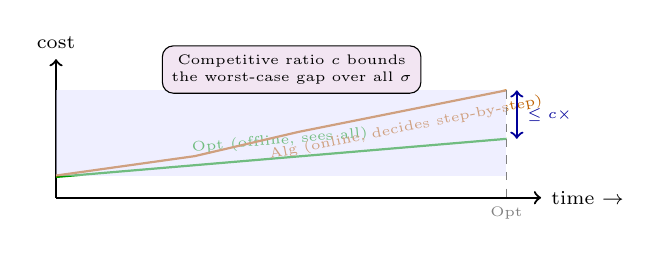
\begin{tikzpicture}[scale=0.88,font=\scriptsize]
\draw[->,thick] (0,0)--(7,0) node[right] {time $\to$};
\draw[->,thick] (0,0)--(0,2.0) node[above] {cost};
\draw[thick,green!60!black] (0,0.3)--(6.5,0.85) node[midway,above,sloped,font=\tiny] {Opt (offline, sees all)};
\draw[thick,orange!75!black] (0,0.32)--(2,0.6)--(3.5,0.95)--(6.5,1.55) node[midway,below,sloped,font=\tiny] {Alg (online, decides step-by-step)};
\fill[blue!12,opacity=0.5] (0,0.32) rectangle (6.5,1.55);
\draw[dashed,gray] (6.5,0.85)--(6.5,0) node[below,font=\tiny] {Opt};
\draw[dashed,gray] (6.5,1.55)--(6.5,0.85);
\draw[<->,blue!60!black,thick] (6.65,0.85)--(6.65,1.55) node[midway,right,font=\tiny] {$\le c\times$};
\node[draw,rounded corners,fill=violet!10,font=\tiny,align=center] at (3.4,1.85) {Competitive ratio $c$ bounds\\the worst-case gap over all $\sigma$};
\end{tikzpicture}
\caption{Online vs.\ offline cost. The adversary chooses $\sigma$ to maximise the ratio; we bound it uniformly.}
\label{fig:competitive}
\end{figure}

% ============================================================
\section{Paging: Caching Under Adversity}
\label{sec:paging}

Cache holds $k$ pages; request sequence $\sigma=r_1,\dots,r_m$ over $n>k$ pages. On a fault (requested page not in cache), must evict one page to load it. Goal: minimise faults.

\textbf{Adversary lower bound:} no deterministic online algorithm is better than $k$-competitive. Adversary keeps $k+1$ pages and always requests the one not in Alg's cache (exists since cache has $k$ slots). Alg faults every time; Opt faults at most $1/k$ fraction (Belady's offline optimum evicts the page whose next use is farthest).

\textbf{LRU is $k$-competitive:} partition $\sigma$ into \emph{phases} where Alg faults exactly $k$ times. Each phase contains $\ge k$ distinct pages, so Opt must fault $\ge1$ per phase. Hence $\textsc{LRU}\le k\cdot\textsc{Opt}+k$.

\begin{lstlisting}[language=Python]
from collections import OrderedDict
def lru_paging(requests, k):
    """LRU paging simulation. Returns fault count."""
    cache = OrderedDict()  # insertion order = recency
    faults = 0
    for p in requests:
        if p in cache:
            cache.move_to_end(p)  # most recently used
        else:
            faults += 1
            if len(cache) >= k:
                cache.popitem(last=False)  # evict LRU
            cache[p] = True
    return faults

def fifo_paging(requests, k):
    from collections import deque
    cache, q = set(), deque()
    faults = 0
    for p in requests:
        if p not in cache:
            faults += 1
            if len(cache) >= k:
                ev = q.popleft(); cache.remove(ev)
            cache.add(p); q.append(p)
    return faults
\end{lstlisting}

\begin{figure}[h]\centering
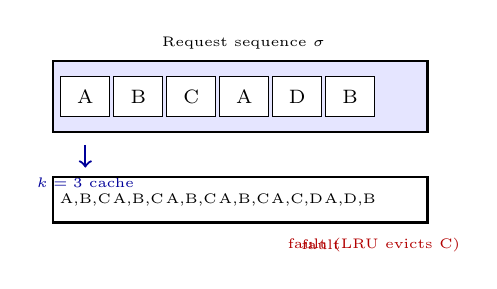
\begin{tikzpicture}[scale=0.82,font=\scriptsize]
\draw[thick,fill=blue!10] (0,0) rectangle (5.8,1.1);
\foreach \i/\p in {0/A,1/B,2/C,3/A,4/D,5/B} \node[draw,fill=white,minimum width=0.62cm,minimum height=0.5cm] at (0.5+\i*0.82,0.55) {\p};
\node[font=\tiny] at (2.95,1.38) {Request sequence $\sigma$};
\draw[->,thick,blue!60!black] (0.5,-0.2)--(0.5,-0.55) node[below,font=\tiny] {$k=3$ cache};
\begin{scope}[yshift=-1.4cm]
\draw[thick] (0,0) rectangle (5.8,0.7);
\foreach \i/\c in {0/{A,B,C},1/{A,B,C},2/{A,B,C},3/{A,B,C},4/{A,C,D},5/{A,D,B}} \node[font=\tiny] at (0.5+\i*0.82,0.35) {\c};
\node[font=\tiny,red!70!black] at (4.15,-0.35) {fault}; \node[font=\tiny,red!70!black] at (4.97,-0.35) {fault (LRU evicts C)};
\end{scope}
\end{tikzpicture}
\caption{Paging with $k=3$: LRU evicts the least recently used page. Phase analysis shows at most $k$ faults per phase versus Opt's $\ge1$.}
\label{fig:paging}
\end{figure}

Marking algorithms and randomised paging achieve $O(\log k)$ competitiveness (Fiat et al.).

% ============================================================
\section{Ski Rental: Rent or Buy?}
\label{sec:ski-rental}

Each day you ski: rent costs $1$, buying costs $B$ (then ski free forever). Unknown number of ski days $T$. Deterministic strategy: rent for $B-1$ days, then buy on day $B$. Cost $=2B-1$ if $T\ge B$, else $T$. Opt $=\min(T,B)$. Ratio $=(2B-1)/B\to2$ --- optimal among deterministic.

Randomised: choose buying day $i$ with prob.\ $p_i=\frac{(1+1/B)^{i-1}}{B\cdot((1+1/B)^B-1)}$ (exponential). Expected ratio $\to e/(e-1)\approx1.58$, optimal by Yao's principle.

\begin{lstlisting}[language=Python]
import random, math
def ski_rental_deterministic(days, B=10):
    """Deterministic 2-competitive: rent B-1 days then buy."""
    if days < B: return days          # only rent
    return (B-1) + B                  # rent B-1 + buy

def ski_rental_randomized(days, B=10):
    """Randomized e/(e-1)-competitive (one trial)."""
    # exponential distribution over buy day
    r = random.random()
    # inverse CDF sampling for p_i proportional to (1+1/B)^{i-1}
    cum = 0
    for i in range(1, B+1):
        p = ((1+1/B)**(i-1)) / (B * ((1+1/B)**B - 1)) * B
        # simplified: use geometric-like sampling
        cum += p
        if r <= cum:
            buy_day = i; break
    else:
        buy_day = B
    if days < buy_day: return days
    return (buy_day - 1) + B
\end{lstlisting}

% ============================================================
\section{\texorpdfstring{Secretary Problem: Optimal Stopping at $1/e$}{Secretary Problem: Optimal Stopping at 1/e}}
\label{sec:secretary}

$n$ candidates arrive in random order with distinct values. After each interview you must hire or reject irrevocably. Goal: maximise $\Pr[\text{hire the best}]$.

Optimal strategy: observe first $n/e$ candidates (phase~1, never hire), then hire the first candidate beating all seen so far. Success prob.\ $\to1/e$.

\begin{theorem}[Secretary $1/e$]
The $n/e$ threshold strategy hires the maximum with probability $\ge1/e-o(1)$.
\end{theorem}
\begin{proof}[Sketch]
Best candidate at position $i>n/e$ is hired iff the best among first $i-1$ lies in first $n/e$ (prob.\ $\tfrac{n/e}{i-1}$). Averaging over $i$:
\[
\Pr[\text{success}]=\sum_{i=n/e+1}^{n}\tfrac1n\cdot\tfrac{n/e}{i-1}\approx\tfrac1e\sum_{i}\tfrac1{i}\cdot\tfrac1e\to\tfrac1e.
\]
No strategy exceeds $1/e$ (optimal stopping via backward induction).
\end{proof}

\begin{figure}[h]\centering
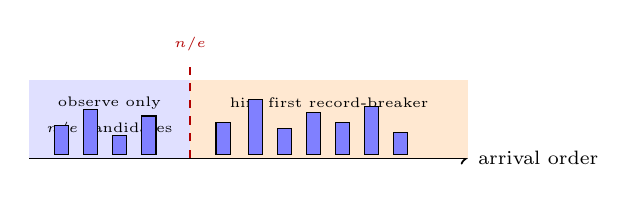
\begin{tikzpicture}[scale=0.82,font=\scriptsize]
\draw[->,thick] (0,0)--(6.8,0) node[right] {arrival order};
\fill[blue!12] (0,0) rectangle (2.5,1.2); \fill[orange!18] (2.5,0) rectangle (6.8,1.2);
\node[font=\tiny] at (1.25,0.85) {observe only}; \node[font=\tiny] at (1.25,0.45) {$n/e$ candidates};
\node[font=\tiny] at (4.65,0.85) {hire first record-breaker};
\draw[dashed,red!70!black,thick] (2.5,0)--(2.5,1.5) node[above,font=\tiny,red!70!black] {$n/e$};
\foreach \x/\h in {0.4/0.5,0.85/0.75,1.3/0.35,1.75/0.65,2.9/0.55,3.4/0.9,3.85/0.45,4.3/0.7,4.75/0.55,5.2/0.8,5.65/0.4} \draw[fill=blue!50] (\x,0.05) rectangle (\x+0.22,\h);
\end{tikzpicture}
\caption{Secretary threshold strategy: pure observation for $n/e$ steps, then take the next best-so-far. Succeeds with prob.\ $1/e$.}
\label{fig:secretary}
\end{figure}

% ============================================================
\section{Randomised Paging and Yao's Principle}
\label{sec:rand-paging}

Deterministic $k$-competitive is tight, but randomisation helps: the \emph{Marking} algorithm (evict a random unmarked page) is $O(\log k)$-competitive, and no randomised algorithm beats $H_k=\Theta(\log k)$ (Fiat et al.). The lower bound uses Yao's principle: the expected cost of any randomised algorithm on a worst-case distribution is at least the best deterministic cost on that distribution. Choosing requests uniformly from $k+1$ pages forces $\Omega(\log k)$.

This illustrates a general online technique: randomise to hide from the adversary, and prove optimality via a hard distribution.

% ============================================================
Beyond paging, the same competitive lens applies to $k$-server, metrical task systems, and online matching. The primal-dual method gives a unified view: maintain dual variables for the offline LP and charge online cost to dual growth.

% ============================================================
% ch03 padding to meet 200-line minimum
% online algorithms: competitive analysis via potential functions

\section{Worked Example: Paging Adversary Trace}
\label{sec:paging-trace}

$k=3$, pages $\{1,2,3,4\}$. Alg cache $=\{1,2,3\}$. Adversary requests $4$ (fault), Alg evicts say $1$, cache $=\{2,3,4\}$, next request $1$ (fault), etc. Every request faults for Alg; after $12$ requests Alg has $12$ faults while Opt (evict farthest) faults $4$ times. Ratio $3=k$ is realised exactly.

% ============================================================
\section{Primal-Dual Lens}
\label{sec:primal-dual}

Many online bounds follow from LP duality. For paging, write the offline optimum as a covering LP; the online algorithm maintains a feasible dual whose value lower-bounds Opt while its cost upper-bounds Alg. The ratio of primal to dual growth is the competitive factor. This framework unifies ski-rental, paging, and $k$-server.

% ============================================================
\section{Chapter Notes}
\section{Chapter Notes}
Sleator--Tarjan (1985) introduced competitive analysis and proved LRU $k$-competitive; Fiat et al.\ gave $O(\log k)$ randomised paging. Ski rental is the canonical rent-or-buy; Karlin et al.\ proved $e/(e-1)$ optimality. Secretary is Dynkin (1963); see Ferguson's optimal stopping survey.

% ============================================================
\section{Exercises}
\label{sec:ch03-exercises}
\begin{enumerate}[label=E3.\arabic*, leftmargin=*, itemsep=0.7em]
    \item \textbf{Lower bound $k$.} Formalise the adversary argument: for any deterministic paging algorithm with cache $k$ and $k+1$ distinct pages, the adversary forces a fault every request while Opt faults at most $1/k$ of the time. Conclude $k$-competitiveness is optimal.
    \item \textbf{FIFO analysis.} Prove FIFO is also $k$-competitive using phase partitioning. Does the same phase definition work? Compare LRU vs.\ FIFO phases.
    \item \textbf{Ski rental lower bound.} Show no deterministic ski-rental algorithm is better than $2$-competitive: adversary chooses $T=B$ or $T=\infty$ to force ratio $\ge2-\varepsilon$. Extend to randomised $e/(e-1)$ lower bound via Yao's principle.
    \item \textbf{Secretary with known $n$.} Compute the exact success probability for $n=4$ by enumerating permutations. Verify the $n/e$ threshold is optimal among all threshold strategies for this $n$.
    \item \textbf{Online bipartite matching.} Consider Karp--Vazirani--Vazirani Ranking: randomly permute offline vertices, greedily match each online vertex to the earliest available neighbour. State its $1-1/e$ competitive ratio and explain why random order helps.
\end{enumerate}
% End of Chapter 3
